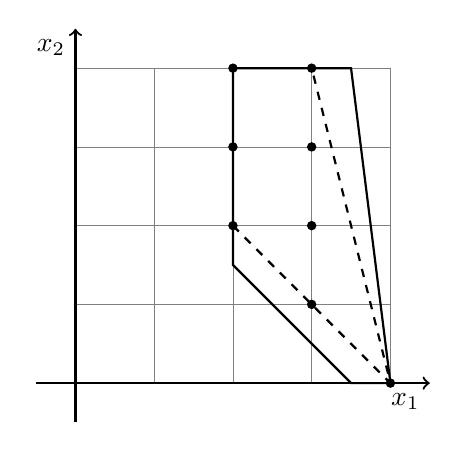
\begin{tikzpicture}
\draw[very thin,gray] (0,0) grid (4,4);
\draw[thick,->] (-0.5,0) -- (4.5,0) node[anchor=north east]{$x_1$};
\draw[thick,->] (0,-0.5) -- (0,4.5) node[anchor=north east]{$x_2$};
\draw[thick] (2,4) -- (2,1.5) -- (3.5,0) -- (4,0) -- (3.5,4) -- cycle;
\draw[thick,dashed] (2,2) -- (4,0) -- (3,4);
\foreach \x/\y in {2/2,2/3,2/4,3/1,3/2,3/3,3/4,4/0} {
  \fill (\x,\y) circle (0.6 mm);
}
\end{tikzpicture}